\section{研究问题}

%%%%%%%%%%%%%%%
\begin{frame}{分布数据一致性问题}
  \begin{columns}[t]
	\column{0.50\textwidth}
	  理想情况:
	  \begin{itemize}
		\item one-size-fits-all 一致性模型
		\item 始终观察到最新副本
	  \end{itemize}
	  \only<1-2>{
	  \begin{center}
		\textcolor{blue}{没有分布数据一致性问题}
	  \end{center}
	  }
	  \only<3->{
	  \begin{center}
		\textcolor{blue}{\soutthick{没有分布数据一致性问题}}
	  \end{center}
	  }
    \pause
	\column{0.50\textwidth}
	  实际情况 (tradeoffs):
	  \fignocaption{width = 0.60\textwidth}{figures/consistency-centric-tradeoff.pdf}
  \end{columns}
  \pause
  \vspace{0.50cm}
  \begin{center}
	\textcolor{red}{分布数据一致性是分布共享数据服务的核心、挑战性问题}
  \end{center}
\end{frame}
%%%%%%%%%%%%%%%
% \begin{frame}{分布数据一致性问题举例 (I)}
%   \fig{width = 0.60\textwidth}{figures/data-inconsistency-comment-reordering.pdf}
%   {社交网络中, 消息-评论乱序 \citeinbeamer{Lloyd}{CACM}{14}.}
% \end{frame}
% %%%%%%%%%%%%%%%
% \begin{frame}{分布数据一致性问题举例 (II)}
%   \begin{figure}[h!]
%     \centering
%     \begin{adjustbox}{max totalsize = {0.65\textwidth}{0.65\textheight}, center}
%       %        File: data-inconsistency-rmw.tex
%     Created: Thu Oct 08 10:00 AM 2015 C
% Last Change: Thu Oct 08 10:00 AM 2015 C
%
\begin{tikzpicture}
  \uncover<1->{
  \begin{scope}
    % phone
    \node (phone) [] at (0,0) {
\includegraphics[scale = 0.4]{figures/phone-icon.png}};
    % tablet
    \node (tablet) [below left = 4.0cm and 3.0cm of phone] {
\includegraphics[scale = 
    0.55]{figures/tablet-icon.jpg}};
    % pc
    \node (pc) [below right = 4.0cm and 3.0cm of phone] {
\includegraphics[scale = 
    0.60]{figures/pc-icon}};
  \end{scope}
  }

    % write from pc 
  \uncover<2->{
    \begin{scope}[<->, blue, line width = 6pt, font = \huge]
      % person at pc
      \only<2>{
      \node (person-pc) [above left = -1.0cm and -2.0cm of pc] {
\includegraphics[scale = 
      0.30]{figures/person-icon}};
      }
      \draw [] (pc.west) to node [midway, sloped, above] {\textbf{1.} update file $f$} 
      (tablet.east);
      \draw [red, loosely dashed] (pc.north) to [out = 90, in = -20] node [midway, sloped, font = 
      \Huge, scale = 2]{$\times$} (phone.east);
      \draw (pc) to [loop, out = 60, in = -10, looseness = 3] node [midway, above, sloped] 
      {\textbf{1.} update file $f$} (pc);
    \end{scope}
   }


    % read from phone
   \uncover<3->{
    \begin{scope}[<->, brown, line width = 6pt, font = \huge]

      % person at phone
      \node (person-phone) [above left = -1.0cm and -2.0cm of phone] {
\includegraphics[scale = 
      0.30]{figures/person-icon}};

      \draw (phone) to [loop, out = 180, in = -100, looseness = 3] node [midway, below, sloped] 
      {\textbf{2.} read file $f$} (phone);   
    \end{scope}

    % update lost
    \node (inconsistency) [font = \huge, right = of person-phone, red] {\bf Update Lost!};
  }
\end{tikzpicture}

%     \end{adjustbox}
%     \caption{多设备文件共享时, 更新丢失 ($\#N = 3, \#W = 2, \#R = 1$).}
%   \end{figure}
% \end{frame}
%%%%%%%%%%%%%%%
\begin{frame}{数据一致性问题研究的历史阶段}
  关于分布数据一致性问题:
  \begin{description}
	\item[基本观点:] 传统问题; 新平台带来新挑战
	\item[我们的工作:] 总结并应对挑战
  \end{description}

  \pause
  \vspace{0.80cm}

  从\textcolor{blue}{``两个方面''}考察研究的历史阶段:
  \vspace{8pt}
  \begin{enumerate}
	\setlength{\itemsep}{6pt}
	\item 理论 vs. 系统
	\item 以数据一致性为核心的 tradeoffs
  \end{enumerate}
\end{frame}
%%%%%%%%%%%%%%%
\begin{frame}{数据一致性问题研究的历史阶段}
  \fignocaption{width = 0.90\textwidth}{figures/consistency-model-history.pdf}
\end{frame}
%%%%%%%%%%%%%%%
%%%%% TODO: draw the history
\begin{frame}{数据一致性问题研究的历史阶段 (多处理器系统)}
  \fig{width = 0.35\textwidth}{figures/consistency-lattice.png}{一致性模型. 依据 \citeinbeamer{Steinke}{JACM}{04} 中 Fig.13 重绘.}

  \begin{center}
	核心 tradeoff: 一致性模型的计算能力 vs. 系统性能
  \end{center}
\end{frame}
%%%%%%%%%%%%%%%
\begin{frame}{数据一致性问题研究的历史阶段 (分布式系统)}
  \graphicspath{{tikz-in-beamer/}}
  \begin{figure}[h!]
    \centering
    \begin{adjustbox}{max totalsize = {1.00\textwidth}{1.00\textheight}, center}
	  %%%%% Description: beamer overlay for history of (weak) consistency models in the context of distributed systems. %%%%%
%%%%% Date: July 25, 2016 %%%%%
%%%%% Author: Hengfeng Wei (hengxin) %%%%

\begin{tikzpicture}[comment/.style = {align = center},
	axis/.style = {dashed, dash pattern = on 8pt off 4pt, line width = 2pt, draw = red},
	sepline/.style = {dashed, line width = 2pt, opacity = 0.80, blue},
    node distance = 2.0cm]

  %%%%%%%%%% Begin: years and papers %%%%%%%%%% 
  % \x: x coordinate; \y: year; \n: name; \lbl: label
  \foreach \x/\y/\n/\lbl in {
	1/1995/eventual/\textcolor{blue}{Eventual consistency},
	6/2000/cap/\textcolor{red}{\bf CAP theorem},
	12/2006/bigtable/\textcolor{blue}{Bigtable@Google},
	18/2007/dynamo/\textcolor{blue}{Dynamo@Amazon},
	25/2012/pacelc/\textcolor{red}{\bf PACELC tradeoff}} {
	\node[star, star points = 5, minimum size = 3pt, draw = red, fill = yellow, line width = 2pt] (\x) at (\x, 5) {};
	\node[below = 0.50cm of \x, font = \large] (\y) {\bf \y};
	\node[above = 0.50cm of \x, align = center, font = \Large] (\n) {\lbl};
  }

  \path[axis] (1) to (6) to (12) to (18) to (25);
  \draw[> = stealth, ->, axis] (25) to (27, 5);
  %%%%%%%%%% End: decades and systems %%%%%%%%%% 
  \draw[sepline] (8, 1) to (8, 10);
  \draw[sepline] (22, 1) to (22, 10);

  \pause
  %%%%% bayou system %%%%%
  \node[below = of 1995] (bayou-fig) {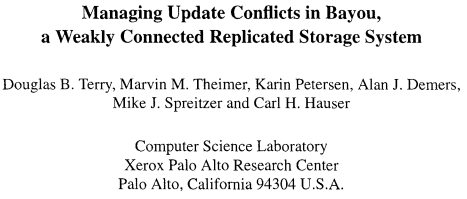
\includegraphics[scale = 0.35]{figs/bayou-paper.png}};
  \node[above = of eventual] (bayou-eventual) {
\includegraphics[scale = 0.13]{figs/24-7-service.png}};

  %%%%% cap theorem %%%%%
  \node[below = of 2000] (cap-ppt) {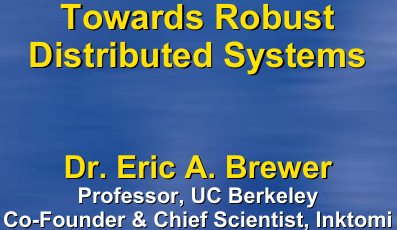
\includegraphics[scale = 0.35]{figs/cap-keynote-ppt.png}};
  % \node[above = of cap] (cap-fig) {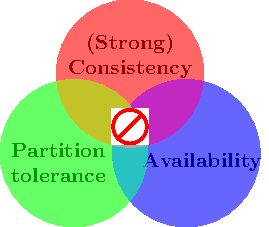
\includegraphics[scale = 0.90]{cap-theorem.pdf}}; 
  \node[above = of cap] (cap-fig) {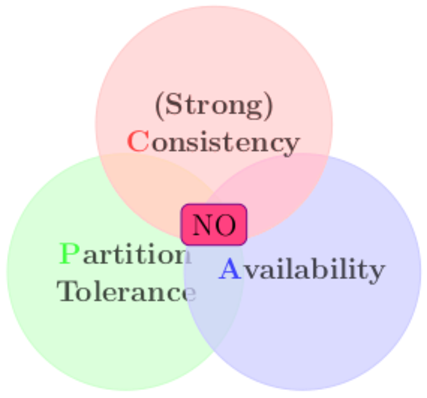
\includegraphics[scale = 0.55]{figs/cap-theorem-no-text.pdf}}; 

  \pause
  %%%%% bigtable %%%%%
  \node[below = of 2006, opacity = 0.80] (bigtable-fig) {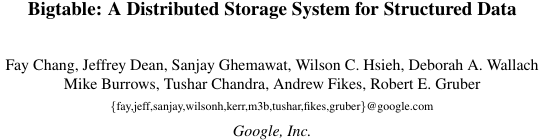
\includegraphics[scale = 0.50]{figs/bigtable-paper.png}};
  \node[above = of bigtable] (bigtable-tradeoff) {
\includegraphics[scale = 0.10]{figs/unavailable.png}};
  
  \pause
  %%%%% dynamo %%%%%
  \node[below = of 2007, opacity = 0.70] (dynamo-fig) {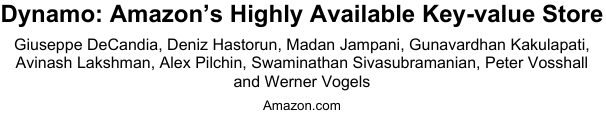
\includegraphics[scale = 0.50]{figs/dynamo-paper.png}};
  \node[above = of dynamo] (dynamo-tradeoff) {
\includegraphics[scale = 0.06]{figs/eventually.jpg}};

  \pause
  %%%%% more systems %%%%%
  \node[] (systems) at ($0.50*(bigtable) + 0.50*(dynamo) + (0, -0.50cm)$) {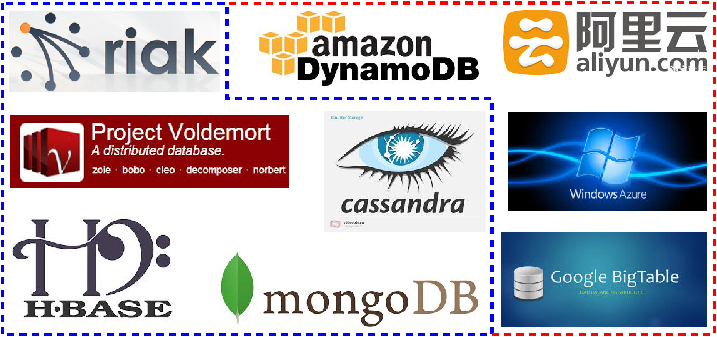
\includegraphics[scale = 0.80]{figs/dsss.pdf}};

  \pause
  %%%%% pacelc tradeoff %%%%%
  \node[below = of 2012] (pacelc-paper) {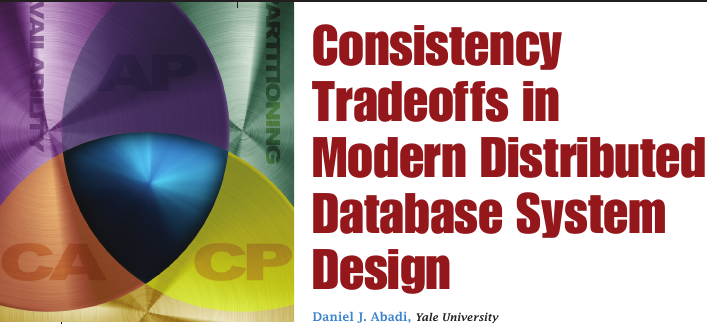
\includegraphics[scale = 0.25]{figs/pacelc-paper.png}};
  \node[above = of pacelc] (pacelc-fig) {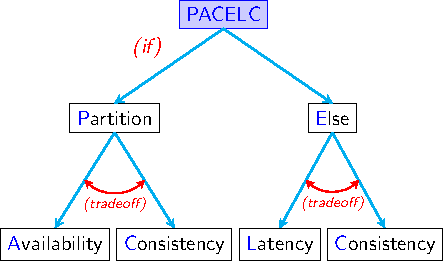
\includegraphics[scale = 0.80]{figs/pacelc-tradeoff-new.pdf}};
\end{tikzpicture}

    \end{adjustbox}
  \end{figure}
\end{frame}
%%%%%%%%%%%%%%%
\begin{frame}{数据一致性问题研究的历史阶段 (结论)}
  \uncover<1->{\textcolor{blue}{新平台的两个特点:}}
  \begin{center}
	\uncover<2->{(1) 云计算新平台凸显应用价值观}

	\uncover<3->{(2) 应用价值观积极拥抱 tradeoffs}
  \end{center}

  \uncover<1->{\textcolor{blue}{需要什么样的数据一致性理论?}}
  \vspace{0.30cm}

  \begin{columns}[t]
	\column{0.50\textwidth}
	  \uncover<2->{
	  (1) 与应用价值观相匹配
	  \fignocaption{width = 0.50\textwidth}{figures/theory-vs-system.pdf}
	  } 
	\column{0.50\textwidth}
	  \uncover<3->{
	 (2) 体现更丰富的 tradeoffs
	  \fignocaption{width = 0.60\textwidth}{figures/consistency-centric-tradeoff.pdf}
	  }
  \end{columns}
\end{frame}
%%%%%%%%%%%%%%%
\begin{frame}{数据一致性问题研究的发展趋势及我们的工作 (I)}
  \begin{columns}[t]
	\column{0.45\textwidth}
	  购物车一致性需求 % \textcolor{blue}{\tiny [Terry@SOSP'13]} % \citeinbeamer{Terry}{SOSP}{13}:
	  \begin{itemize}
		\item 优先 \textcolor{blue}{\texttt{\small read-my-writes}}
		\item 可接受 \textcolor{blue}{\texttt{\small any consistency}} 只要延迟低于300ms
	  \end{itemize}
	\column{0.55\textwidth}
	  出租车实时位置查询一致性需求:
	  \begin{itemize}
		\item 所有读请求都要满足 \textcolor{blue}{\texttt{\small 2-atomicity}}
		\item 违反 \textcolor{blue}{\texttt{\small atomicity}} 的读请求低于$1\%$ 
	  \end{itemize}
  \end{columns}

  \pause
  \vspace{1.00cm}

  \textcolor{red}{应用价值观导向的数据一致性理论:}
  \begin{enumerate}
	\item 多样化, 可调节
	\item 精细化, 可度量
  \end{enumerate}
\end{frame}
%%%%%%%%%%%%%%%
\begin{frame}{数据一致性问题研究的发展趋势及我们的工作 (II)}
  \begin{description}
	\setlength{\itemsep}{10pt}
	\item[多样化:] 从单一到融合 (mono- vs. multi-) \citeinbeamer{Terry}{CACM}{13} 
	  \vspace{5pt}
	  \begin{itemize}
		\setlength{\itemsep}{5pt}
		\item 融合强弱一致性: 不同操作, 不同一致性需求 
		\item 融合一致与不一致: 容忍``有限度''的不一致
	  \end{itemize}
	  \begin{columns}
		\column{0.50\textwidth}
		  \fignocaption{width = 0.50\textwidth}{figures/tradeoff.jpg} 
		\column{0.50\textwidth}
		  \fignocaption{width = 0.35\textwidth}{figures/one-size-fit-all-text.jpg} 
	  \end{columns}
	\pause
	\item[可调节:] think \textcolor{red}{\it dynamically} \citeinbeamer{Terry}{SOSP}{13}
	  \vspace{10pt}
	  \begin{center}
	    依据应用需求/系统状态调节数据一致性
	  \end{center}
  \end{description}
\end{frame}
%%%%%%%%%%%%%%%
\begin{frame}{数据一致性问题研究的发展趋势及我们的工作 (III)}
  \begin{description}
	\setlength{\itemsep}{20pt}
	\item[精细化:] 从二元到连续谱 \citeinbeamer{Yu}{TOCS}{02}
	  \begin{columns}
		\column{0.50\textwidth}
		  % \fignocaption{scale = 0.06}{figures/coin-flip.jpg}
		  \fignocaption{scale = 0.15}{figures/black-or-white.jpg}
		\column{0.50\textwidth}
		  \fignocaption{scale = 0.05}{figures/prism-spectrum.jpg}
	  \end{columns}
	  \pause
	\item[可度量:] think \textcolor{red}{\it probabilistically} \citeinbeamer{Brewer}{PODC}{00}
	  \fignocaption{width = 0.25\textwidth}{figures/tape-measure.jpg}
	  \begin{center}
		量化系统执行, 后验系统对一致性的满足程度
	  \end{center}
  \end{description}
\end{frame}
%%%%%%%%%%%%%%%
\begin{frame}{数据一致性问题研究的发展趋势及我们的工作 (III)}
  \begin{columns}[t]
	\column{0.50\textwidth}
	  2个理念:
	  \begin{enumerate}
		\item 多样化, 可调节
		\item 精细化, 可度量
	  \end{enumerate}
	\column{0.50\textwidth}
      3份工作:
	  \begin{enumerate}
		\item VPC
		\item PA2AM
		\item RVSI
	  \end{enumerate}
  \end{columns}
\end{frame}
%%%%%%%%%%%%%%%
